\subsection{\bf Class Separability with Code Change Embeddings (RQ3)}
\label{sec:separation}

%\subsubsection{\bf Contribution of Code Change Embeddings in Classification (RQ3)}

\begin{figure*}[t]
	\centering
	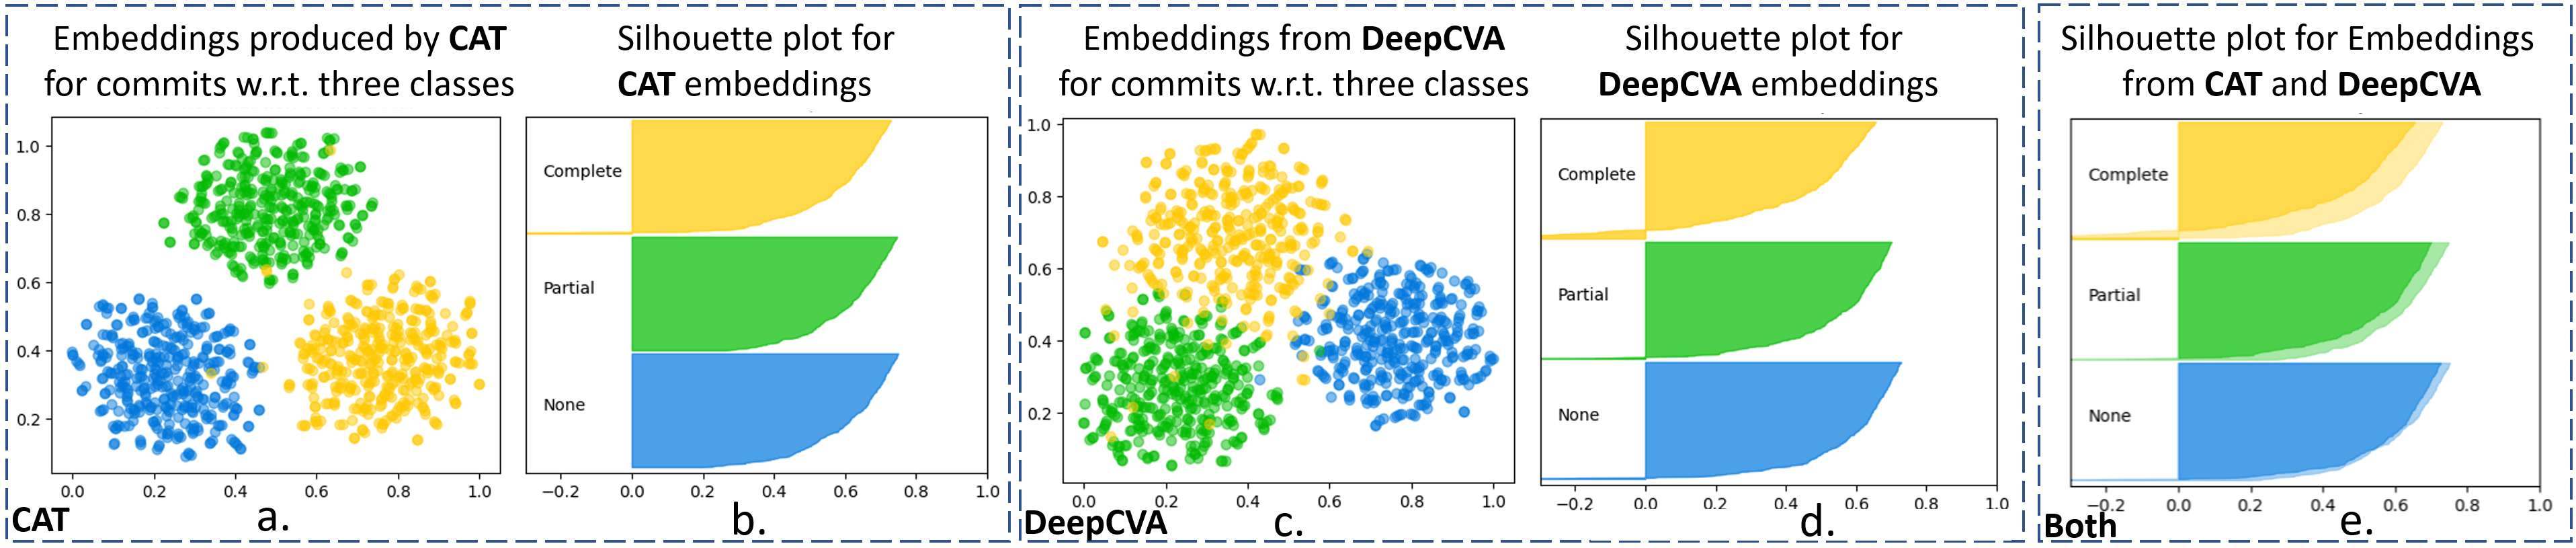
\includegraphics[width=6.9in]{graphs/confidentiality}
        \vspace{-6pt}
	\caption{Silhouette Plots for the Embeddings of Commits produced by {\tool} and DeepCVA on CONFIDENTIALITY (RQ3)}
	\label{fig:confidentiality}
\end{figure*}

\begin{figure*}[t]
	\centering
	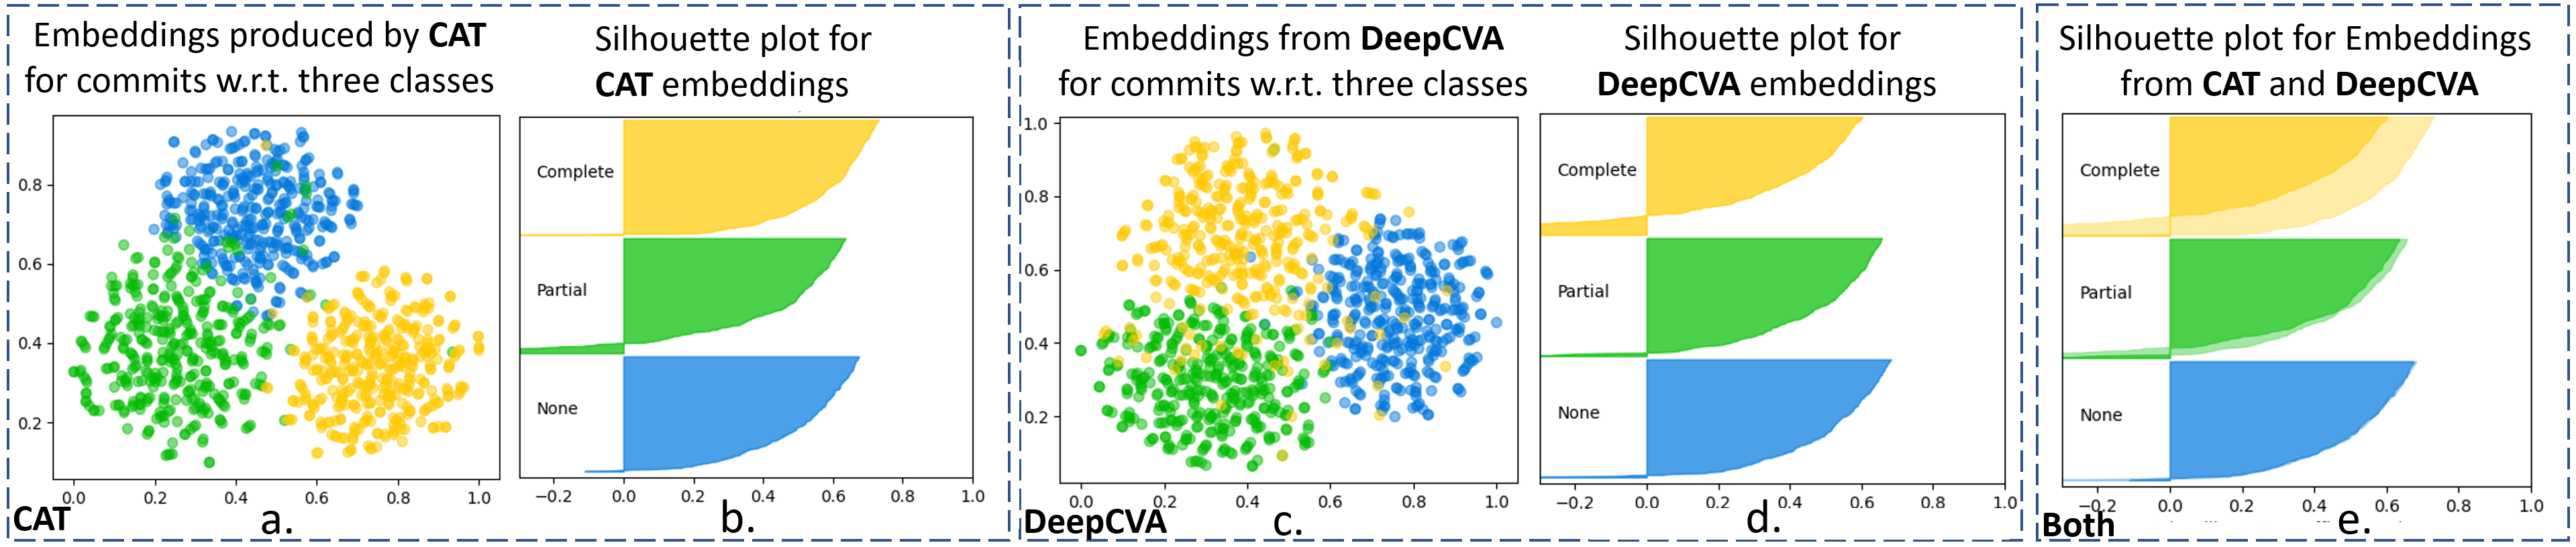
\includegraphics[width=6.9in]{graphs/integrity}
        \vspace{-6pt}
	\caption{Silhouette Plots for the Embeddings of Commits produced by {\tool} and DeepCVA on INTEGRITY (RQ3)}
	\label{fig:integrity}
\end{figure*}

\begin{figure*}[t]
	\centering
	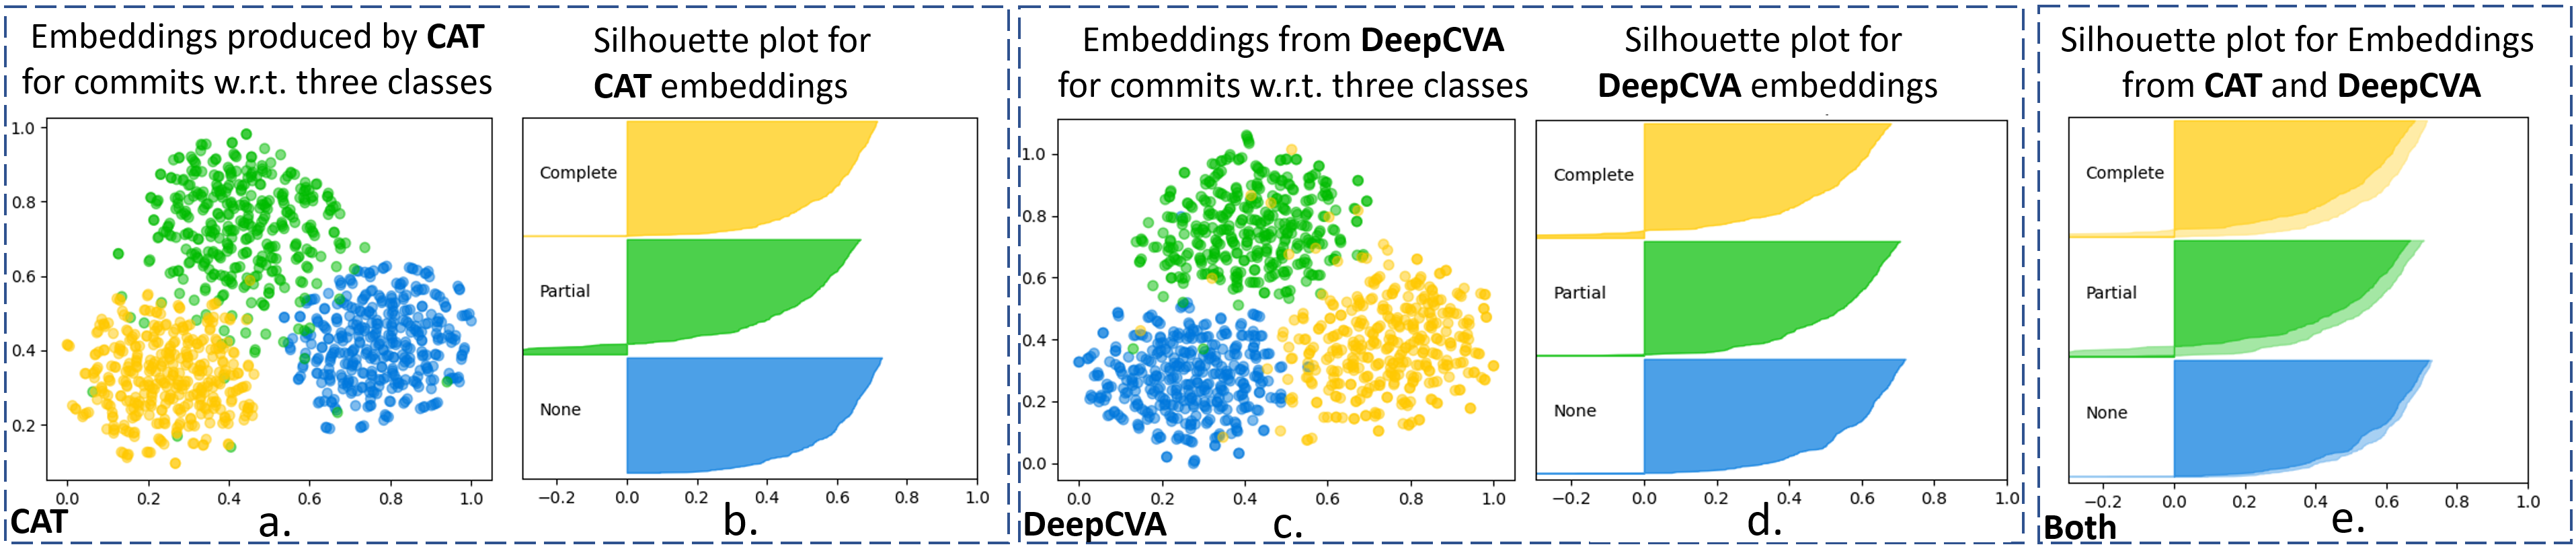
\includegraphics[width=6.9in]{graphs/availability}
       \vspace{-6pt}
	\caption{Silhouette Plots for the Embeddings of Commits produced by {\tool} and DeepCVA on AVAILABLITY (RQ3)}
	\label{fig:availability}
\end{figure*}

%
%\begin{figure*}[t]
%	\centering
%	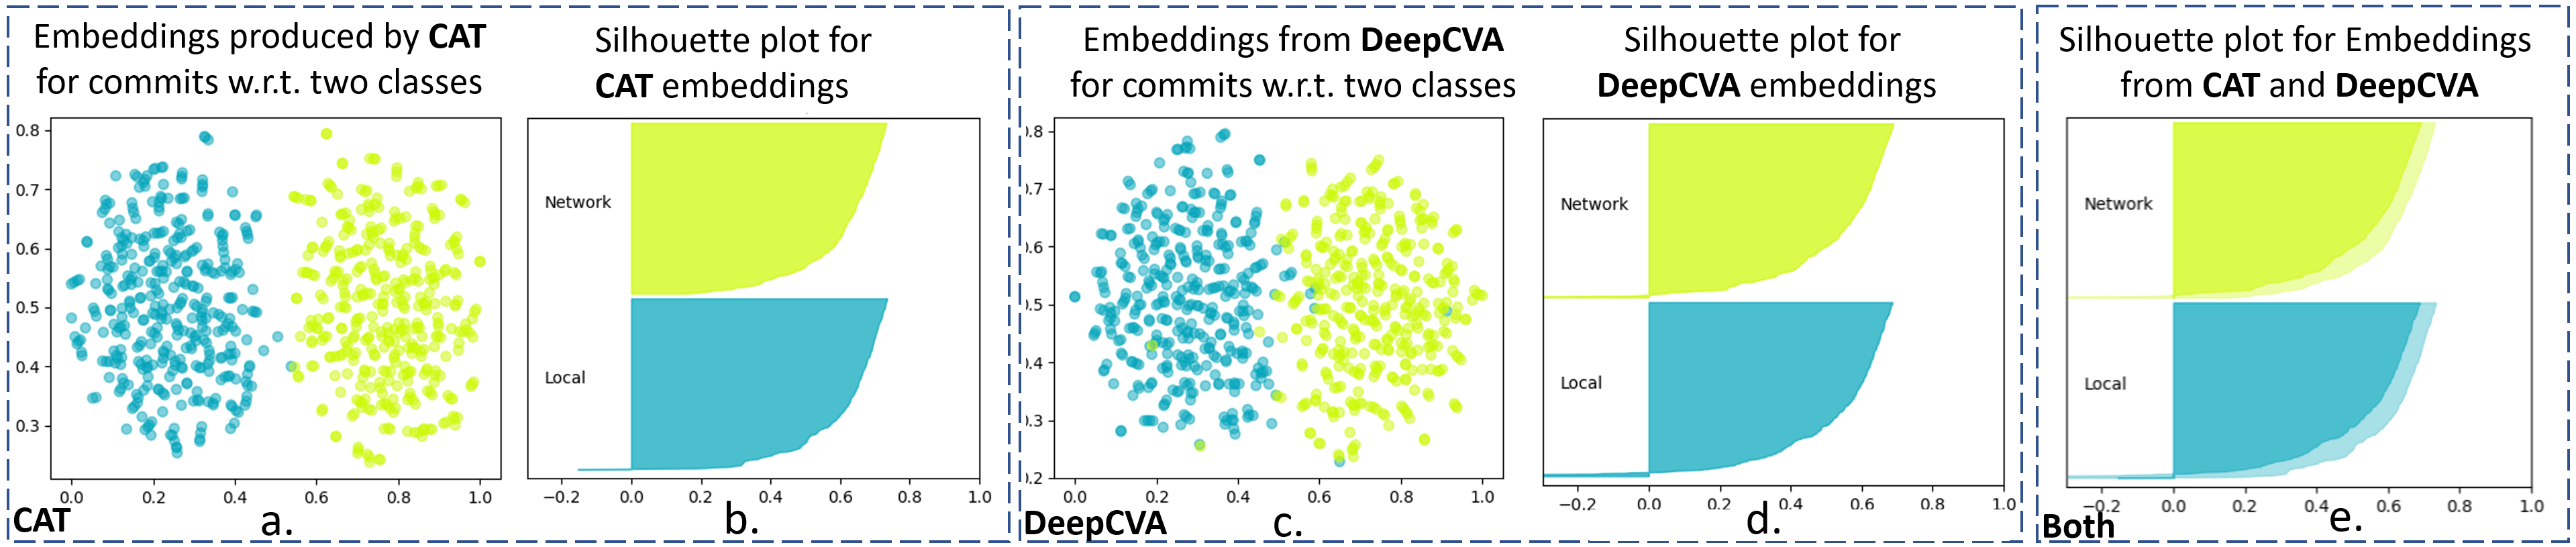
\includegraphics[width=6.9in]{graphs/access-vector}
%        \vspace{-6pt}
%	\caption{Silhouette Plots for the Embeddings of Commits produced by {\tool} and DeepCVA regarding ACCESS VECTOR}
%	\label{fig:access-vector}
%\end{figure*}

%\begin{figure*}[t]
%	\centering
%	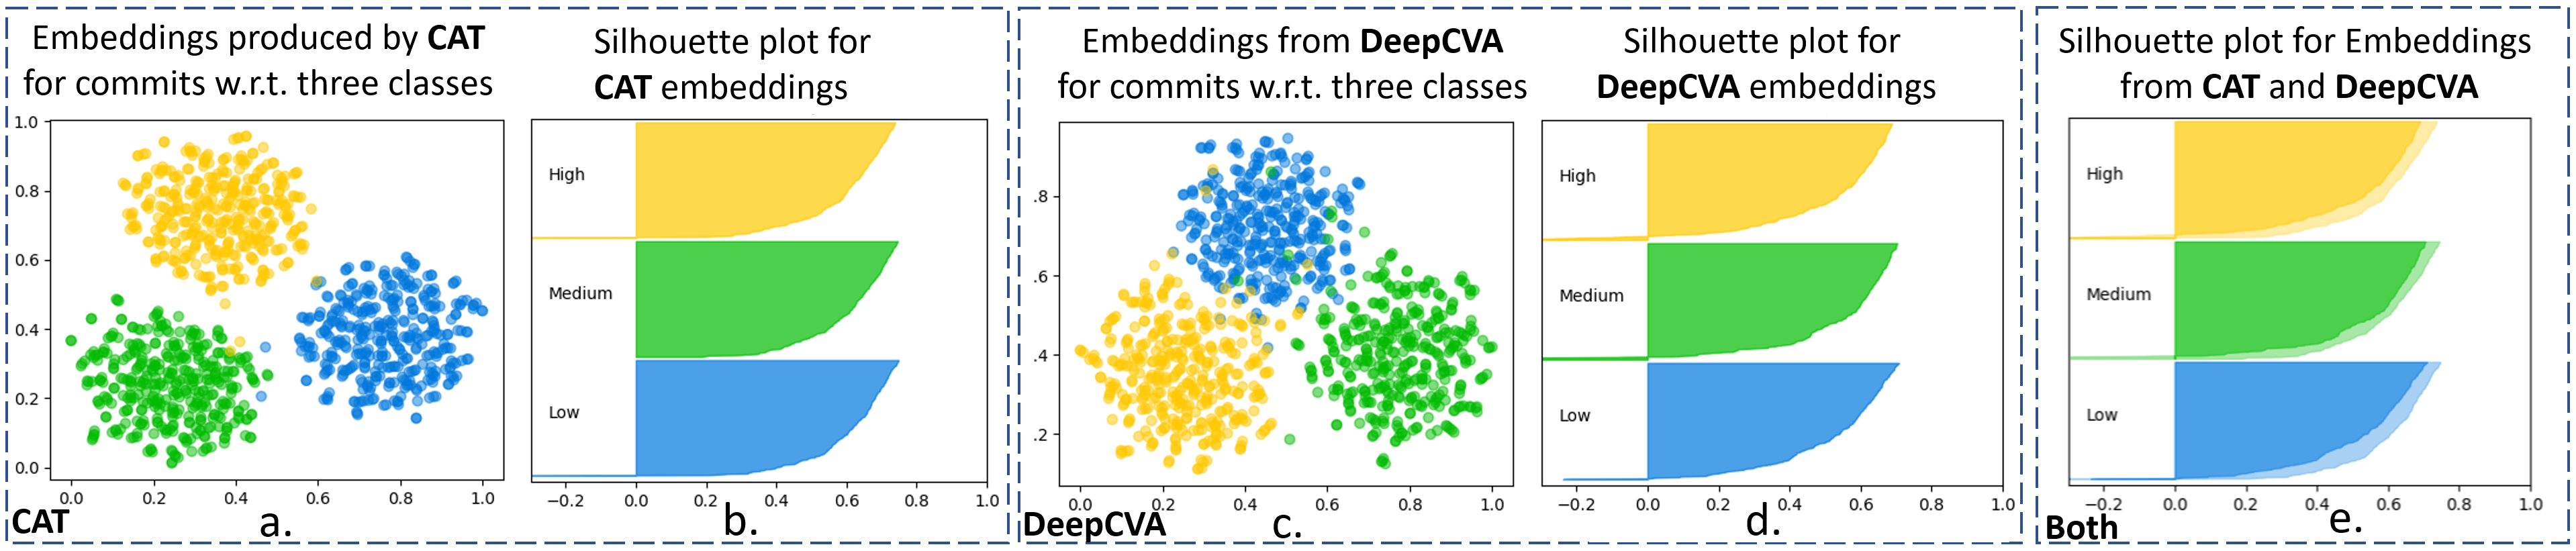
\includegraphics[width=6.9in]{graphs/access-complexity}
%        \vspace{-6pt}
%	\caption{Silhouette Plots for the Embeddings of Commits produced by {\tool} and DeepCVA regarding ACCESS COMPLEXITY}
%	\label{fig:access-complexity}
%\end{figure*}

%\begin{figure*}[t]
%	\centering
%	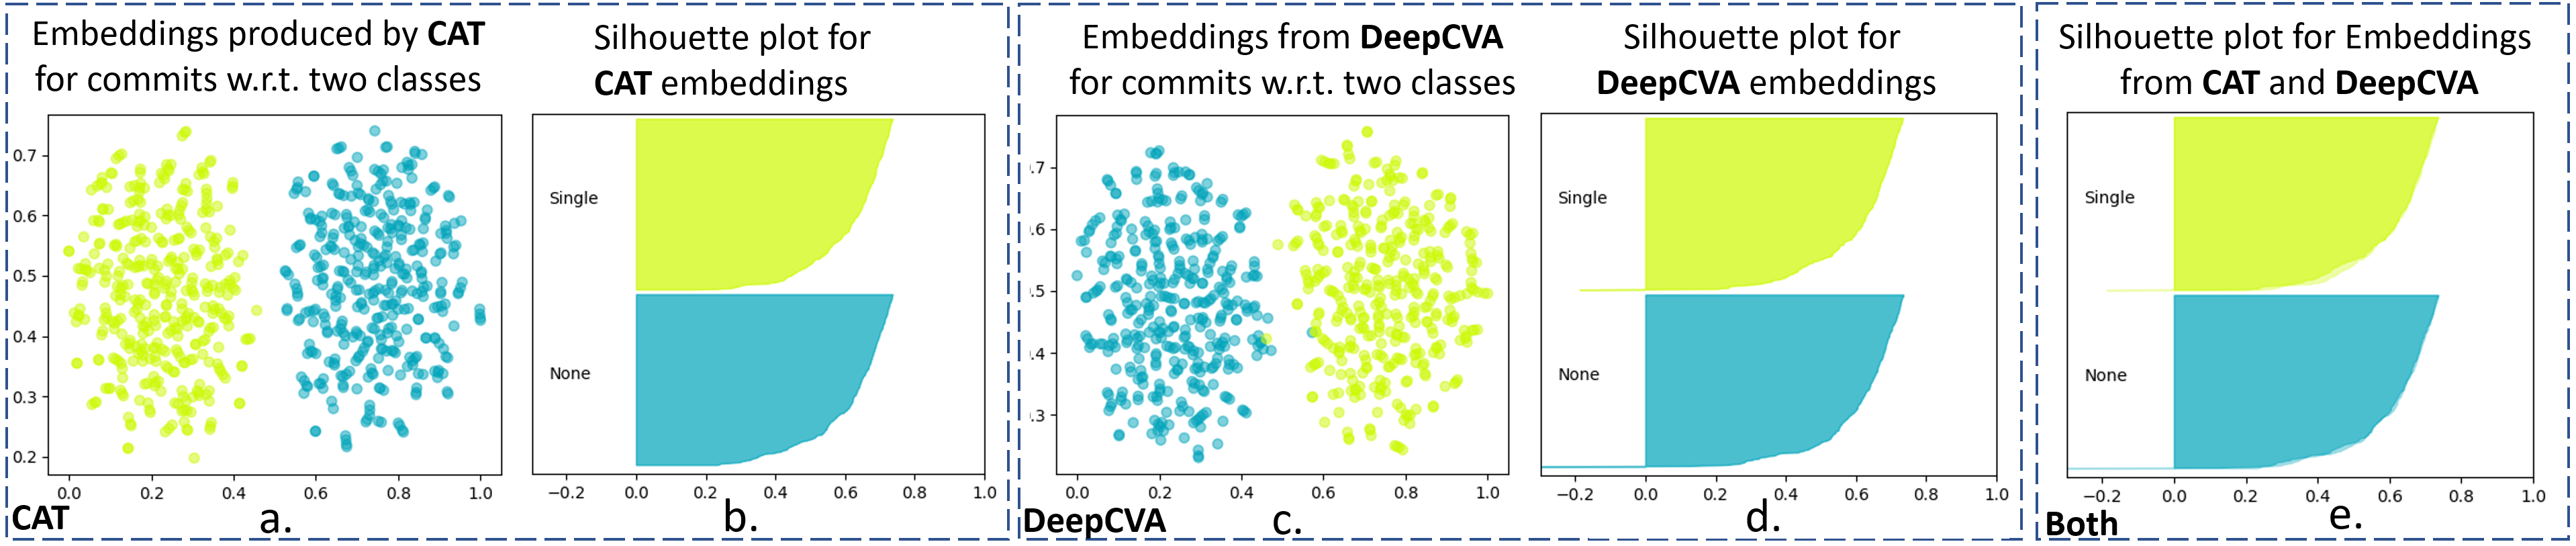
\includegraphics[width=6.9in]{graphs/authentication}
%        \vspace{-6pt}
%	\caption{Silhouette Plots for the Embeddings of Commits produced by {\tool} and DeepCVA regarding AUTHENTICATION}
%	\label{fig:authentication}
%\end{figure*}

%\begin{figure*}[t]
%	\centering
%	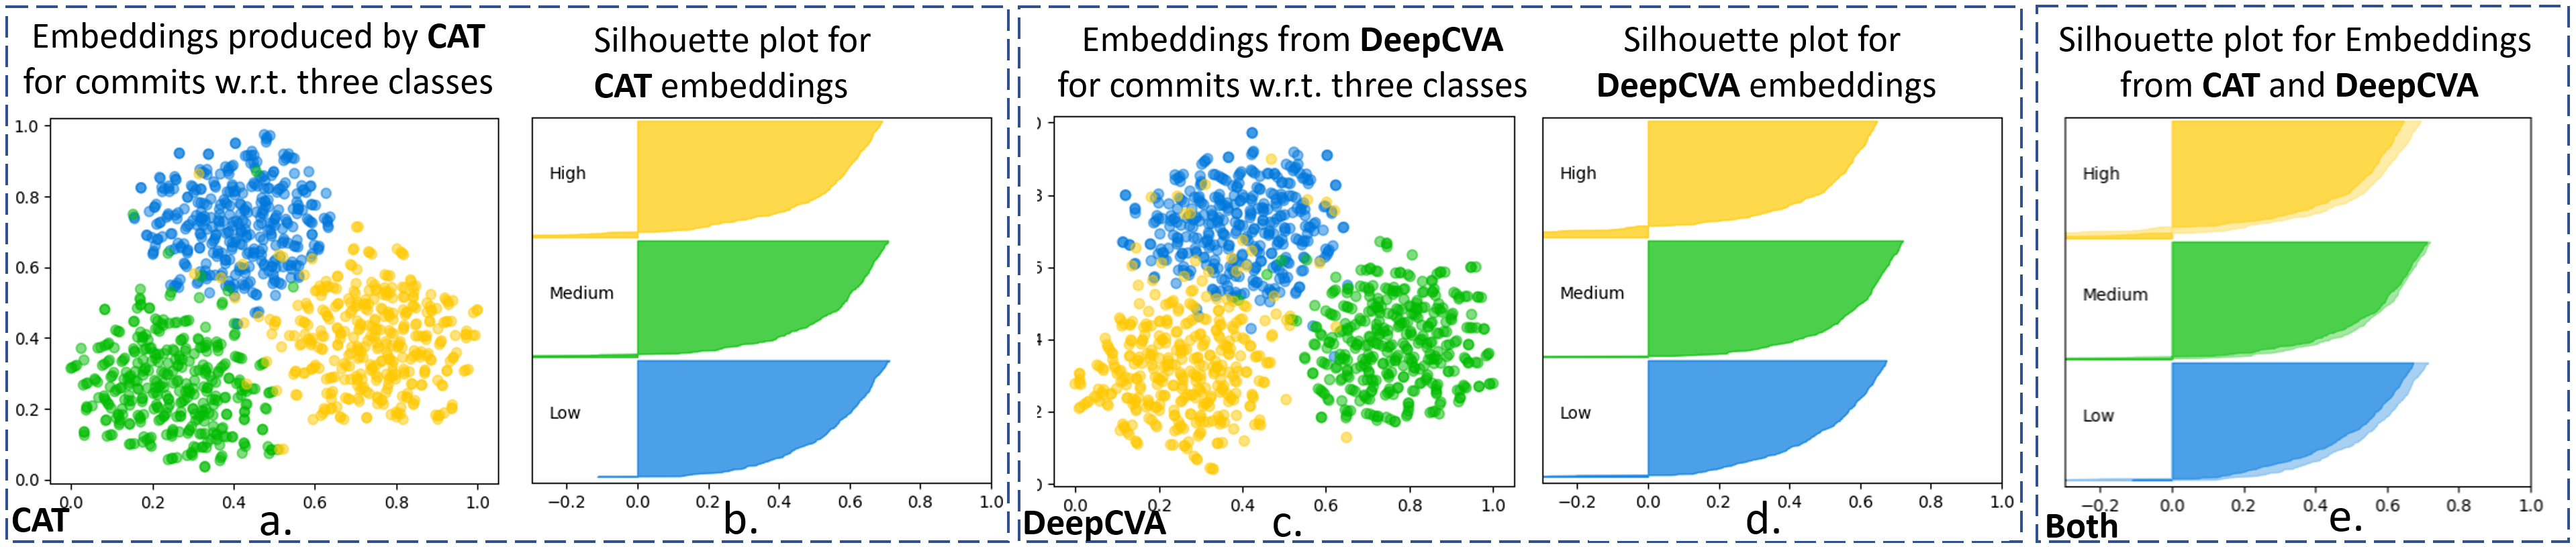
\includegraphics[width=6.9in]{graphs/severity}
%        \vspace{-6pt}
%	\caption{Silhouette Plots for the Embeddings of Commits produced by {\tool} and DeepCVA regarding SEVERITY}
%	\label{fig:severity}
%\end{figure*}

%We first processed each vulnerability assessment type (VAT).

In this study, we aim to show that our {\em embeddings for code
changes helps {\tool} have better class-separation}, i.e., {\em better
classification measures} for detection and assessment than that of the baseline.

%In this experiment, we aim to show that our novel graph-based, code
%change embeddings help {\tool} perform better classification for the
%grades in vulnerability assessment types than the $n$-gram-based
%embeddings in the baseline approach. We aim to show that the
%embeddings from {\tool} helps it have better class-separation, leading
%to better detection/assessment.

For each class~$C$ regarding a vulnerability assessment type (VAT), we
selected 366 commits that are labeled with the class $C$ in the
oracle. This was chosen based on the population of the data, such that the sample size corresponded to a 95\% confidence level, with a confidence interval of 5\% for each VAT. 
For example, for {\em Confidentiality}, we randomly selected
an equal number of commits (i.e., 366), that are marked as {\em None}, {\em Partial}, and {\em Complete}.
%Since our study
%does not depend on the distribution across classes, we chose the same
%number of samples for a class. The sample size, i.e., 366, was chosen based on the population of our data, and a , and a corresponding confidence interval of 
For each type, we took those 366 $\times$ 3 = 1,098 commits and used
{\em {\tool}'s code change representation learning model} and {\em DeepCVA's
$n$-gram-based embedding model} to produce the embeddings for
those commits.  We projected the embeddings from these approaches
into the vector space using t-SNE~\cite{tsne} technique, based on which we can visualize high-dimensional data by giving
each data point its projected location in a two-dimensional vector
space. Next, in the silhouette plots~\cite{silhouette-plot}, we succinctly present the data points for these embeddings, which represent how well they have
been classified.

Figure~\ref{fig:confidentiality} shows the comparison between the
silhouette plots for the embeddings produced by {\tool} and DeepCVA
regarding 3 classes of
Confidentiality. Figures~\ref{fig:confidentiality}a. and c. display
the t-SNE visualizations for the embeddings, while
%produced by {\tool} and DeepCVA, respectively.
figures~\ref{fig:confidentiality}b. and d. display the silhouette
plots for the data in these visualizations.
%for {\tool} and DeepCVA.
The silhouette coefficient value ($X$-axis in
Figures~\ref{fig:confidentiality}b., d., e.) is a measure of how
similar an object is to its own class compared to~other classes, which ranges from [-1, 1]. Here, a higher value
indicates that an object is well matched to~its own class and poorly
matched to neighboring classes. If most objects have high values, the
class configuration is proper. That corresponds
to better-formed classes, facilitating a model to group the commits
into the correct classes (i.e., {\em None, Partial,} and {\em Complete}).
If many points have low or negative values, the
class configuration is ill-formed, i.e. does not help with
classification.

Let us consider the commits in the {\em Complete} class
in~Figures \ref{fig:confidentiality}a. and b. Each line in {\em
Complete} class in Figure~\ref{fig:confidentiality}b. corresponds to a
point in {\em Complete} class in the vector space in
Figure~\ref{fig:confidentiality}a. Length of a line is equal to
the silhouette coefficient for a point. These lines are
sorted from largest to smallest, and drawn from top to bottom, creating
a knife shape. As seen, the knife shapes from DeepCVA have longer and thicker
tails than those from {\tool}, which actually have no tail for the
classes {\em Partial} and {\em None}. 
%This means that DeepCVA produces
%those embeddings that are not well-matched with its own classes and
%mixed with the embeddings of the neighboring classes. 
%This means that 
Thus, DeepCVA produces embeddings that overlap more with their
neighboring classes.  In Figure~\ref{fig:confidentiality}e., we place
two silhouette plots in an overlay image. The plot from {\tool} is
thicker than that from DeepCVA: {\tool} produces more points with
positive values than DeepCVA. In brief,
Figures~\ref{fig:confidentiality}a--e show that the {\em embeddings
for code changes from {\tool} facilitates better classification for
vulnerability assessment than the embeddings produced by DeepCVA}.

%~\ref{fig:access-vector},
%~\ref{fig:access-complexity},
%~\ref{fig:authentication},

%Figures~\ref{fig:integrity},~\ref{fig:availability},
%and~\ref{fig:severity}

Figure~\ref{fig:integrity} and Figure~\ref{fig:availability} show the
comparison among the silhouette plots for the embeddings from {\tool}
and DeepCVA on {\em Integrity} and {\em Availability} (remaining VAT
types are not shown here due to space limit). We can see that the
comparisons for all VATs have the same trend, i.e., the knife shapes
from {\tool} have no or shorter tails, and are thicker than those of
DeepCVA. In brief, the silhouette plots indicate that {\tool} produces
embeddings that have more cohesion with the ones in the same class and
more separation with the ones in the different classes. Thus, our {\bf
  embeddings with more class-separability help {\tool} perform better
  classification}.
%for vulnerability assessment}.

%regarding each vulnerability assessment type}.


\begin{figure}[t]
	\centering
	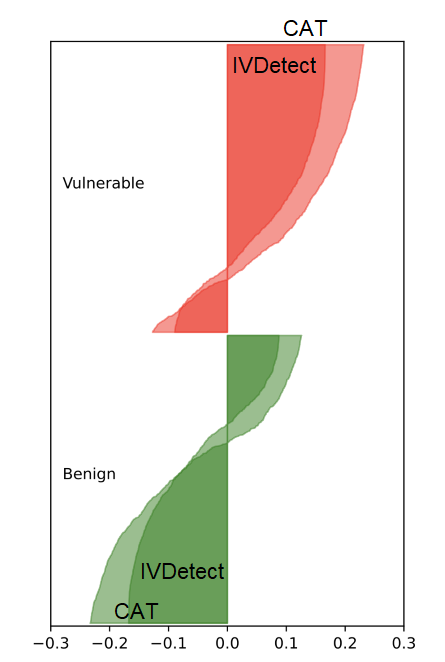
\includegraphics[width=1.3in]{graphs/plot-vd}
       \vspace{-6pt}
	\caption{Silhouette Plots for the Embeddings of Commits produced by {\tool} and IVDetect for Vulnerability Detection: {\tool} has better Class Separability (RQ3)}
	\label{fig:vd}
\end{figure}

We also performed the same plotting for the classification task for
vulnerability detection. Considering the overlap between two plots in
Figure~\ref{fig:vd}, the knife shapes from {\tool} for both classes
(vulnerability and benign) are wider and have less negative values
than those from the best baseline IVDetect. Specifically, the average
silhouette score in {\tool} is 0.027, while that of IVDetect is
0.0072. Thus, {\tool} has better class-separability, leading to better
performance.
